\chapter{CAPÍTULO 3}
\section{Exemplo de Tabelas, Quadros e Figuras}

{\centering\bfseries\color{red}
Exemplo de Tabela
\par}

\begin{table}[ht]
\centering
\caption{Preços de alimentos em dólares de 1900-1952 a
1995-1997}
\begin{supertabular}{m{3.6cm}m{3.7cm}m{3.6cm}m{3.0cm}}
\hline
\multicolumn{1}{m{3.636cm}|}{\centering{ ALIMENTO}} &
\multicolumn{1}{m{3.741cm}|}{\centering{ 1950-1952}} &
\multicolumn{1}{m{3.635cm}|}{\centering{ 1995-1977}} &
\centering\arraybslash{ VARIAÇÃO PERCENTUAL}\\\hline
\centering{ Trigo} &
\centering{ 427,6} &
\centering{ 159,3} &
\centering\arraybslash{ {}-62,7}\\
\centering{ Arroz} &
\centering{ 789,7} &
\centering{ 282,3} &
\centering\arraybslash{ {}-64,2}\\
\centering{ Sorgo} &
\centering{ 328,7} &
\centering{ 110,9} &
\centering\arraybslash{ {}-66,2}\\
\centering{ Milho} &
\centering{ 372,0} &
\centering{ 119,1} &
\centering\arraybslash{ {}-68,0}\\\hline
\end{supertabular}
    \legend{Fonte: Sen (2000, p. 240). }
    \label{tab:alimentos}
\end{table}

\bigskip

{\centering\bfseries\color{red}
Exemplo de Quadro
\par}

\begin{quadro}[htb]
\centering
\caption{Comparativo de competitividade}
\begin{supertabular}{|m{2.5cm}|m{2.5cm}|m{6.0cm}|m{3.0cm}|}
\hline
{ EMPRESA } &
{ PRINCIPAL MATÉRIA-PRIMA } &
{ ALTERNATIVAS DE SUPRIMENTOS PARA A PRINCIPAL MATÉRIA-PRIMA } &
{ FLEXIBILIDADE }\\\hline
{ Copesul } &
{ Nafta } &
{ Disponibilidade de produto na Argentina} &
{ 45\% condensado e GLP }\\\hline
{ Copene } &
{ Nafta } &
{ Alternativas Venezuela e Argélia } &
{ Inexistente }\\\hline
{ PQU } &
{ Nafta } &
{ Único fornecedor } &
{ Inexistente }\\\hline
{ Rio Polímeros } &
{ Etano } &
{ Único fornecedor } &
{ Inexistente }\\\hline
{ Baía Blanca } &
{ Etano } &
{ Projeto Mega / Única opção } &
{ Inexistente }\\\hline
\end{supertabular}
    \legend{Fonte: Freire e Jardim (2000, p. 78)}
    \label{quad:quadro1}
\end{quadro}

\bigskip
\clearpage

{\centering\bfseries\color{red}
Exemplo de Gráfico
\par}
\begin{figure}[ht]
    \centering
    \caption{Acesso à internet 1999 – 2002}
    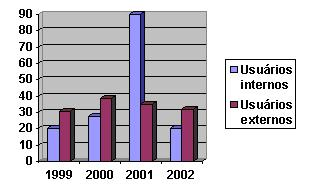
\includegraphics[width=12.5cm,height=7.2cm]{ModeloMonografiaDCCUFRJ-img002.png} 
    \legend{Fonte: Silva, Camargo Pires (2004, p. 45)}
    \label{fig:internet}
\end{figure}

\clearpage
\section{Exemplos de Citações}
{\centering\bfseries\color{red}
Exemplos de Citações
\par}

{\centering\bfseries\color{red}
Citação direta:
\par}

\bigskip

Citações diretas de até 3 linhas, devem iniciar e terminar por aspas duplas.\\

Se o texto original já contiver aspas duplas, substituí-las por aspas simples. A indicação da fonte da citação pode
estar inserida no texto ou após a citação.\\

\bigskip

{\color{red}
Exemplo:}

\bigskip

Segundo Castro (2001, p. 23): {\textquotedbl}Os deveres da conduta do anestesiologista constituem predicados importantes
quando se quer avaliar a qualidade do procedimento.{\textquotedbl}\\

\bigskip

{\color{red}
ou}

\bigskip

{
{\textquotedbl}A expressão 'furiosa' dessa estátua de que fala Rebelais, corresponde também à realidade.{\textquotedbl}
(BAKHTIN, 1987, p. 89).}

\bigskip

{\centering\bfseries\color{red}
Citação Direta com mais de três linhas:
\par}

\bigskip

As citações diretas, no texto, com mais de três linhas, devem ser
destacadas com recuo de 4 cm da margem esquerda, com letra menor que a do texto utilizado e sem as aspas. A indicação da fonte da citação pode estar inserida no texto ou após a citação. \\ 

\bigskip

{\color{red}
Exemplo:}
\bigskip
Sobre mercado financeiro, Fortuna (1996, p. 15) considera:\\
\bigskip

\begin{citacao}
O mercado financeiro permite que um agente econômico qualquer, sem perspectivas de aplicação, em algum empreendimento
próprio, da poupança que é capaz de gerar, seja colocado em contato com outro, cujas perspectivas de investimento
superam as respectivas disponibilidades de poupança.\\
\end{citacao}

\bigskip
A seguir uma citação em inglês:\\

\begin{citacao}[english]
This text is an example in English language in italic with correct hyphenation. This text is an example in English language in italic with correct hyphenation. This text is an example in English language in italic with correct hyphenation.
\end{citacao}
\bigskip

\clearpage{\centering\bfseries\color{red}
Citação Indireta:
\par}

\bigskip

Não se utilizam aspas para esse tipo de citação, nem a(s) página(s) de onde foi extraída a ideia.\\

\bigskip

{\color{red}
Exemplo:}

\bigskip

A bíblia começou a ser escrita no ano 1.000 a.C. e foi finalizada em 100 d.C., com a morte do último apóstolo, São João, levando aproximadamente 1.150 anos para ser concluída \cite{book:GHELLER}.\\


\bigskip

{\centering\bfseries\color{red}
Citação de Citação:
\par}

\bigskip

A indicação da fonte é feita pelo sobrenome do autor da obra citada (não consultada), ano, seguido da expressão latina apud. Após, indica-se o sobrenome do autor da obra consultada, seguido do ano de publicação, precedido por vírgula. Quando for citação direta incluir a(s) página(s) após a data de publicação, precedida de vírgula.\\

\bigskip

{\sffamily
\textrm{\textcolor{red}{Exemplo no texto}}\textrm{:}}

\bigskip

{\sffamily
\textrm{citado por }}

\bigskip

{\sffamily
\textrm{Segundo Marques e Ribeiro}\footnote{\ MARQUES, Alberto; RIBEIRO, \textbf{Angela. As fazendas agrícolas}. São
Paulo: Ática, 2000. 350 p.}\textrm{ (2000 }\textrm{\textcolor{black}{apud }}\textrm{OLIVEIRA, 2001), \apudonline {art:PRADO}{book:AMADO} o Serviço de
Atenção Médico-Sanitário da Suécia tem uma tradição de mais de cem anos. }}

\bigskip

{\color{red}
ou}

{\sffamily
\textrm{\textcolor{red}{Em nota de rodapé}}\textrm{:}}

\bigskip

{\centering\bfseries\color{red}
Indicação da Citação:
\par}

\bigskip

{\sffamily
\textrm{Se a indicação da fonte da citação estiver incluída na frase, a mesma deve aparecer apenas com a inicial
maiúscula seguida de parênteses, com a data de publicação do }\textrm{documento. Quando for citação direta incluir a(s)
página(s) após a data de publicação, precedida de vírgula.}}

\bigskip

{\color{red}
Exemplo com autor pessoal:}

\bigskip

Segundo Fonseca(2004, p. 36): {\textquotedbl}Se não houver mecanismos jurídicos que assegurem a proteção dos direitos
humanos, esse valor não será concretizado pelo Poder Público.{\textquotedbl}\\

\bigskip

{\sffamily
\textrm{\textcolor{red}{Exemplo com dois autores: }}}

\bigskip

Tonetto e Reck (2001, p. 134) destacam: {\textquotedbl}Este autoconhecimento pressupõe conhecer seus limites
[...]{\textquotedbl} \\

\bigskip

{\color{red}
Exemplo com mais de três autores:}

\bigskip

Neste contexto, Couto e outros (2004, p. 52) destacam que: {\textquotedbl}No capitalismo não é a simples ausência do
patrão que promove a superação do despotismo da divisão laboral.{\textquotedbl}\\

\bigskip

{\sffamily
\textrm{\textcolor{red}{Exemplo com autor institucional: }}}

\bigskip

De acordo com a Pontifícia Universidade Católica do Rio Grande do Sul (2001, p. 24): {\textquotedbl}[...] no horizonte 2001/2010, o esforço estratégico da PUCRS será centrado em sete áreas estratégicas [...]{\textquotedbl}\\

\bigskip

{\color{red}
Exemplo sem autor(es), com a entrada pelo título:}

\bigskip

Segundo o Guia de clareamento dental (1996, p. 8): {\textquotedbl}A causa mais comum do escurecimento dental é o tratamento endodôntico realizado de modo inadequado e sem os cuidados técnicos.{\textquotedbl}\\

\bigskip

{\color{red}
Exemplo sem autor(es), com a entrada pelo título que inicia por artigo:}

\bigskip

O movimento social, com o intuito de realizar uma transformação social, é uma das tarefas mais importantes da atualidade
(O COOPERATIVISMO..., 2002).\\

\bigskip

As citações a seguir foram colocadas para que as referências aparecessem na bibliografia. Como exemplo temos os livro de Jorge Amado \cite{book:AMADO}  \cite{book:AMADO2}, e este autor que desconheço \cite{book:OHANSSON}, além de \cite{book:ENGEL} e um artigo \cite{art:PRADO}. Notem que é gerado um link hipertexto no documento em PDF.
